\documentclass[11pt,oneside]{article}
\usepackage[T1]{fontenc}
\usepackage[utf8]{inputenc}
% \usepackage{lmodern}
%\usepackage[adobe-utopia,uppercase=upright,greeklowercase=upright]{mathdesign}
\usepackage[adobe-utopia]{mathdesign}
%\usepackage{minionpro}
% \usepackage{pifont}
% \usepackage{amssymb}
\usepackage{amsmath}
\usepackage[francais]{babel}
% \usepackage[francais]{varioref}
\usepackage[dvips]{graphicx}

\usepackage{framed}
\usepackage[normalem]{ulem}
\usepackage{fancyhdr}
\usepackage{titlesec}
\usepackage{vmargin}
\usepackage{longtable}

\usepackage{ifthen}


%\usepackage{epsfig}
\usepackage{subfig}

\usepackage{multirow}
\usepackage{multicol} % Portions de texte en colonnes
\usepackage{flafter}%floatants après la référence



\usepackage{color}
\usepackage{colortbl}


\definecolor{gris25}{gray}{0.75}
\definecolor{bleu}{RGB}{18,33,98}
\definecolor{bleuf}{RGB}{42,94,171}
\definecolor{bleuc}{RGB}{231,239,247}
\definecolor{rougef}{RGB}{185,18,27}
\definecolor{rougec}{RGB}{255,230,231}
\definecolor{vertf}{RGB}{103,126,82}
\definecolor{vertc}{RGB}{220,255,191}
\definecolor{violetf}{RGB}{112,48,160}
\definecolor{violetc}{RGB}{230,224,236}

\newenvironment{sci}[1][\hsize]%
{%
    \def\FrameCommand%
    {%
%\rotatebox{90}{\textit{\textsf{Scilab}}\includegraphics[height=.8cm]{png/logo_scilab}} 
\rotatebox{90}{\includegraphics[height=.6cm]{png/logo_scilab}} 
        {\color{violetf}\vrule width 3pt}%
        \hspace{0pt}%must no space.
        \fboxsep=\FrameSep\colorbox{violetc}%
    }%
    \MakeFramed{\hsize #1 \advance\hsize-\width\FrameRestore}%
}%
{\endMakeFramed}%

\newenvironment{pseudo}[1][\hsize]%
{%
    \def\FrameCommand%
    {%
\rotatebox{90}{\textit{\textsf{Pseudo Code}}} 
        {\color{violetf}\vrule width 3pt}%
        \hspace{0pt}%must no space.
        \fboxsep=\FrameSep\colorbox{violetc}%
    }%
    \MakeFramed{\hsize #1 \advance\hsize-\width\FrameRestore}%
}%
{\endMakeFramed}%

\newenvironment{py}[1][\hsize]%
{%
    \def\FrameCommand%
    {%
%\rotatebox{90}{\textit{\textsf{Python}}} 
\rotatebox{90}{\includegraphics[height=.6cm]{png/logo_python}} 
        {\color{violetf}\vrule width 3pt}%
        \hspace{0pt}%must no space.
        \fboxsep=\FrameSep\colorbox{violetc}%
    }%
    \MakeFramed{\hsize #1 \advance\hsize-\width\FrameRestore}%
}%
{\endMakeFramed}%


\newenvironment{corrige}[1][\hsize]%
{%
    \def\FrameCommand
    {%
\rotatebox{90}{\textit{\textsf{Correction}}} 
        {\color{violetf}\vrule width 3pt}%
        \hspace{0pt}%must no space.
        \fboxsep=\FrameSep\colorbox{violetc}%
    }%
    \MakeFramed{\hsize#1\advance\hsize-\width\FrameRestore}%
}%
{\endMakeFramed}%



\newenvironment{rem}[1][\hsize]%
{%
    \def\FrameCommand
    {%
\rotatebox{90}{\textit{\textsf{Remarque}}} 
        {\color{bleuf}\vrule width 3pt}%
        \hspace{0pt}%must no space.
        \fboxsep=\FrameSep\colorbox{bleuc}%
    }%
    \MakeFramed{\hsize#1\advance\hsize-\width\FrameRestore}%
}%
{\endMakeFramed}%


\newenvironment{savoir}[1][\hsize]%
{%
    \def\FrameCommand
    {%
\rotatebox{90}{\textit{\textsf{Savoir}}} 
        {\color{bleuf}\vrule width 3pt}%
        \hspace{0pt}%must no space.
        \fboxsep=\FrameSep\colorbox{bleuc}%
    }%
    \MakeFramed{\hsize#1\advance\hsize-\width\FrameRestore}%
}%
{\endMakeFramed}%

\newenvironment{prob}[1][\hsize]%
{%
    \def\FrameCommand%
    {%
\rotatebox{90}{\textit{\textsf{ Problématique}}} 
        {\color{rougef}\vrule width 3pt}%
        \hspace{0pt}%must no space.
        \fboxsep=\FrameSep\colorbox{rougec}%
    }%
    \MakeFramed{\hsize#1\advance\hsize-\width\FrameRestore}%
}%
{\endMakeFramed}%

\newenvironment{obj}[1][\hsize]%
{%
    \def\FrameCommand%
    {%
\rotatebox{90}{\textit{\textsf{ $\;$}}} 
        {\color{rougef}\vrule width 3pt}%
        \hspace{0pt}%must no space.
        \fboxsep=\FrameSep\colorbox{rougec}%
    }%
    \MakeFramed{\hsize#1\advance\hsize-\width\FrameRestore}%
}%
{\endMakeFramed}%

\newenvironment{defi}[1][\hsize]%
{%
    \def\FrameCommand%
    {%
\rotatebox{90}{\textit{\textsf{Définition\\}}} 
        {\color{bleuf}\vrule width 3pt}%
        \hspace{0pt}%must no space.
        \fboxsep=\FrameSep\colorbox{bleuc}%
    }%
    \MakeFramed{\hsize#1\advance\hsize-\width\FrameRestore}%
}%
{\endMakeFramed}%


\newenvironment{demo}[1][\hsize]%
{%
    \def\FrameCommand%
    {%
\rotatebox{90}{\textit{\textsf{Démonstration\\}}} 
        {\color{bleuf}\vrule width 3pt}%
        \hspace{0pt}%must no space.
        \fboxsep=\FrameSep\colorbox{bleuc}%
    }%
    \MakeFramed{\hsize#1\advance\hsize-\width\FrameRestore}%
}%
{\endMakeFramed}%


\newenvironment{hypo}[1][\hsize]%
{%
    \def\FrameCommand%
    {%
\rotatebox{90}{\textit{\textsf{Hypothèse\\}}} 
        {\color{bleuf}\vrule width 3pt}%
        \hspace{0pt}%must no space.
        \fboxsep=\FrameSep\colorbox{bleuc}%
    }%
    \MakeFramed{\hsize#1\advance\hsize-\width\FrameRestore}%
}%
{\endMakeFramed}%


\newenvironment{prop}[1][\hsize]%
{%
    \def\FrameCommand%
    {%
\rotatebox{90}{\textit{\textsf{Propriété\\}}} 
        {\color{bleuf}\vrule width 3pt}%
        \hspace{0pt}%must no space.
        \fboxsep=\FrameSep\colorbox{bleuc}%
    }%
    \MakeFramed{\hsize#1\advance\hsize-\width\FrameRestore}%
}%
{\endMakeFramed}%

\newenvironment{props}[1][\hsize]%
{%
    \def\FrameCommand%
    {%
\rotatebox{90}{\textit{\textsf{Propriétés\\}}} 
        {\color{bleuf}\vrule width 3pt}%
        \hspace{0pt}%must no space.
        \fboxsep=\FrameSep\colorbox{bleuc}%
    }%
    \MakeFramed{\hsize#1\advance\hsize-\width\FrameRestore}%
}%
{\endMakeFramed}%

\newenvironment{exemple}[1][\hsize]%
{%
    \def\FrameCommand%
    {%
\rotatebox{90}{\textit{\textsf{Exemple\\}}} 
        {\color{vertf}\vrule width 3pt}%
        \hspace{0pt}%must no space.
        \fboxsep=\FrameSep\colorbox{vertc}%
    }%
    \MakeFramed{\hsize#1\advance\hsize-\width\FrameRestore}%
}%
{\endMakeFramed}%

\newenvironment{resultat}[1][\hsize]%
{%
    \def\FrameCommand%
    {%
\rotatebox{90}{\textit{\textsf{Résultat\\}}} 
        {\color{rougef}\vrule width 3pt}%
        \hspace{0pt}%must no space.
        \fboxsep=\FrameSep\colorbox{rougec}%
    }%
    \MakeFramed{\hsize#1\advance\hsize-\width\FrameRestore}%
}%
{\endMakeFramed}%

\newenvironment{methode}[1][\hsize]%
{%
    \def\FrameCommand%
    {%
\rotatebox{90}{\textit{\textsf{Méthode\\}}} 
        {\color{rougef}\vrule width 3pt}%
        \hspace{0pt}%must no space.
        \fboxsep=\FrameSep\colorbox{rougec}%
    }%
    \MakeFramed{\hsize#1\advance\hsize-\width\FrameRestore}%
}%
{\endMakeFramed}%

\newenvironment{theo}[1][\hsize]%
{%
    \def\FrameCommand%
    {%
\rotatebox{90}{\textit{\textsf{Théorème\\}}} 
        {\color{rougef}\vrule width 3pt}%
        \hspace{0pt}%must no space.
        \fboxsep=\FrameSep\colorbox{rougec}%
    }%
    \MakeFramed{\hsize#1\advance\hsize-\width\FrameRestore}%
}%
{\endMakeFramed}%

\newenvironment{warn}[1][\hsize]%
{%
    \def\FrameCommand%
    {%
\rotatebox{90}{\textit{\textsf{Attention\\}}} 
        {\color{rougef}\vrule width 3pt}%
        \hspace{0pt}%must no space.
        \fboxsep=\FrameSep\colorbox{rougec}%
    }%
    \MakeFramed{\hsize#1\advance\hsize-\width\FrameRestore}%
}%
{\endMakeFramed}%

% \usepackage{pstricks}
%\usepackage{minitoc}
% \setcounter{minitocdepth}{4}

\setcounter{tocdepth}{2}

% \mtcselectlanguage{french} 

%\usepackage{draftcopy}% "Brouillon"
% \usepackage{floatflt}
\usepackage{psfrag}
%\usepackage{listings} % Permet d'insérer du code de programmation
\renewcommand{\baselinestretch}{1.2}

% Changer la numérotation des figures :
% ------------------------------------
% \makeatletter
% \renewcommand{\thefigure}{\ifnum \c@section>\z@ \thesection.\fi
%  \@arabic\c@figure}
% \@addtoreset{figure}{section}
% \makeatother
 


%%%%%%%%%%%%
% Définition des vecteurs %
%%%%%%%%%%%%
 \newcommand{\vect}[1]{\overrightarrow{#1}}

%%%%%%%%%%%%
% Définition des torseusr %
%%%%%%%%%%%%

 \newcommand{\torseur}[1]{%
\left\{{#1}\right\}
}

\newcommand{\torseurcin}[3]{%
\left\{\mathcal{#1} \left(#2/#3 \right) \right\}
}

\newcommand{\torseurstat}[3]{%
\left\{\mathcal{#1} \left(#2\rightarrow #3 \right) \right\}
}

 \newcommand{\torseurc}[8]{%
%\left\{#1 \right\}=
\left\{
{#1}
\right\}
 = 
\left\{%
\begin{array}{cc}%
{#2} & {#5}\\%
{#3} & {#6}\\%
{#4} & {#7}\\%
\end{array}%
\right\}_{#8}%
}

 \newcommand{\torseurcol}[7]{
\left\{%
\begin{array}{cc}%
{#1} & {#4}\\%
{#2} & {#5}\\%
{#3} & {#6}\\%
\end{array}%
\right\}_{#7}%
}

 \newcommand{\torseurl}[3]{%
%\left\{\mathcal{#1}\right\}_{#2}=%
\left\{%
\begin{array}{l}%
{#1} \\%
{#2} %
\end{array}%
\right\}_{#3}%
}

 \newcommand{\vectv}[3]{%
\vect{V\left( {#1} \in {#2}/{#3}\right)}
}


\newcommand{\vectf}[2]{%
\vect{R\left( {#1} \rightarrow {#2}\right)}
}

\newcommand{\vectm}[3]{%
\vect{\mathcal{M}\left( {#1}, {#2} \rightarrow {#3}\right)}
}


 \newcommand{\vectg}[3]{%
\vect{\Gamma \left( {#1} \in {#2}/{#3}\right)}
}

 \newcommand{\vecto}[2]{%
\vect{\Omega\left( {#1}/{#2}\right)}
}
% }$$\left\{\mathcal{#1} \right\}_{#2} =%
% \left\{%
% \begin{array}{c}%
%  #3 \\%
%  #4 %
% \end{array}%
% \right\}_{#5}}

%  ------------------------------------------
% | Modification du formatage des sections : | 
%  ------------------------------------------

% Grands titres :
% ---------------

\newcommand{\titre}[1]{%
\begin{center}
      \bigskip
      \rule{\textwidth}{1pt}
      \par\vspace{0.1cm}
      
      \textbf{\large #1}
      \par\rule{\textwidth}{1pt}
    \end{center}
    \bigskip
  }

% Supprime le numéro du chapitre dans la numérotation des sections:
% -----------------------------------------------------------------
\makeatletter
\renewcommand{\thesection}{\@arabic\c@section}
\makeatother


% \titleformat{\chapter}[display]
% {\normalfont\Large\filcenter}
% {}
% {1pc}
% {\titlerule[1pt]
%   \vspace{1pc}%
%   \Huge}[\vspace{1ex}%
% \titlerule]


%%%% Chapitres Comme PY Pechard %%%%%%%%%
% numéro du chapitre
\DeclareFixedFont{\chapnumfont}{OT1}{phv}{b}{n}{80pt}
% pour le mot « Chapitre »
\DeclareFixedFont{\chapchapfont}{OT1}{phv}{m}{it}{40pt}
% pour le titre
\DeclareFixedFont{\chaptitfont}{T1}{phv}{b}{n}{25pt}

\definecolor{gris}{gray}{0.75}
\titleformat{\chapter}[display]%
	{\sffamily}%
	{\filleft\chapchapfont\color{gris}\chaptertitlename\
	\\
	\vspace{12pt}
	\chapnumfont\thechapter}%
	{16pt}%
	{\filleft\chaptitfont}%
	[\vspace{6pt}\titlerule\titlerule\titlerule]

%%%%  Fin Chapitres Comme PY Pechard %%%%%%%%%


% Section, subsection, subsubsection sans serifs :
% % ----------------------------------------------

% \makeatletter
% \renewcommand{\section}{\@startsection{section}{0}{0mm}%
% {\baselineskip}{.3\baselineskip}%
% {\normalfont\sffamily\Large\textbf}}%
% \makeatother

\makeatletter
\renewcommand{\@seccntformat}[1]{{\textcolor{bleu}{\csname
the#1\endcsname}\hspace{0.5em}}}
\makeatother

\makeatletter
\renewcommand{\section}{\@startsection{section}{1}{\z@}%
                       {-4ex \@plus -1ex \@minus -.4ex}%
                       {1ex \@plus.2ex }%
                       {\normalfont\Large\sffamily\bfseries}}%
\makeatother
 
\makeatletter
\renewcommand{\subsection}{\@startsection {subsection}{2}{\z@}
                          {-3ex \@plus -0.1ex \@minus -.4ex}%
                          {0.5ex \@plus.2ex }%
                          {\normalfont\large\sffamily\bfseries}}
\makeatother
 
\makeatletter
\renewcommand{\subsubsection}{\@startsection {subsubsection}{3}{\z@}
                          {-2ex \@plus -0.1ex \@minus -.2ex}%
                          {0.2ex \@plus.2ex }%
                          {\normalfont\large\sffamily\bfseries}}
\makeatother
 
\makeatletter             
\renewcommand{\paragraph}{\@startsection{paragraph}{4}{\z@}%
                                    {-2ex \@plus-.2ex \@minus .2ex}%
                                    {0.1ex}%               
{\normalfont\sffamily\bfseries}}
\makeatother
 

\makeatletter             
\renewcommand{\subparagraph}{\@startsection{subparagraph}{5}{\z@}%
                                    {-2ex \@plus-.2ex \@minus .2ex}%
                                    {0.1ex}%               
{\normalfont\bfseries Question }}
\makeatother

\renewcommand{\thesubparagraph}{\arabic{subparagraph}} 
%
\makeatletter
%\renewcommand{\subparagraph}{\@startsection{subparagraph}{5}{\z@}%
%                                       {-2ex \@plus-.1ex \@minus .2ex}%
%                                       {0.1ex}%
%				    {\normalfont\normalsize\sffamily\bfseries}}
%\makeatletter
% \makeatletter
% \renewcommand{\subsection}{\@startsection{subsection}{1}{2mm}%
% {\baselineskip}{.3\baselineskip}%
% {\normalfont\sffamily\large\textbf}}%
% \makeatother
% 
% \makeatletter
% \renewcommand{\subsubsection}{\@startsection{subsubsection}{2}{4mm}%
% {\baselineskip}{.15\baselineskip}%
% {\normalfont\sffamily\large\textbf}}%
% \makeatother
% 
% \makeatletter
% \renewcommand{\paragraph}{\@startsection{paragraph}{3}{6mm}%
% {\baselineskip}{.15\baselineskip}%
% {\normalfont\sffamily\large\textbf}}%
% \makeatother
 
\setcounter{secnumdepth}{5}


%  --------
% | Marges |
%  --------


% \setmarginsrb{2.5cm}{1.5cm}{2.5cm}{2cm}{1cm}{1cm}{1cm}{1cm}
\setmarginsrb{1.5cm}{1cm}{1cm}{1.5cm}{1cm}{1cm}{1cm}{1cm}

% Changer les marges localement :
% -----------------------------
\newenvironment{changemargin}[2]{\begin{list}{}{%
\setlength{\topsep}{0pt}%
\setlength{\leftmargin}{0pt}%
\setlength{\rightmargin}{0pt}%
\setlength{\listparindent}{\parindent}%
\setlength{\itemindent}{\parindent}%
\setlength{\parsep}{0pt plus 1pt}%
\addtolength{\leftmargin}{#1}%
\addtolength{\rightmargin}{#2}%
}\item }{\end{list}}



\usepackage{pst-solides3d}
\usepackage{titletoc}
\titlecontents{chapter}[+3pc]
  {\addvspace{10pt}\sffamily\bfseries}
{\contentslabel[{\pscirclebox[fillstyle=solid,fillcolor=gray!25,
linecolor=gray!25,framesep=4pt]{\textcolor{white}{\thecontentslabel}}}]{2.5pc}}
  {}
  {\dotfill \normalfont\thecontentspage\ }

\titlecontents{section}[3pc]
  {\addvspace{2pt}\sffamily}
  {\contentslabel[\thecontentslabel]{1.8pc}}
  {}
  {\dotfill \normalfont\thecontentspage\ }

\titlecontents{subsection}[5pc]
  {\addvspace{2pt}\sffamily}
  {\contentslabel[\thecontentslabel]{1.8pc}}
  {}
  {\dotfill \normalfont\thecontentspage\ }

\titlecontents{subsubsection}[8pc]
  {\addvspace{2pt}\sffamily}
  {\contentslabel[\thecontentslabel]{3pc}}
  {}
  {\dotfill \normalfont\thecontentspage\ }
%{\;\titlerule\;\normalfont\thecontentspage\ }

\titlecontents{paragraph}[9pc]
  {\addvspace{2pt}\sffamily}
  {\contentslabel[\thecontentslabel]{3.5pc}}
  {}
  {\dotfill \normalfont\thecontentspage\ }




\usepackage[%
    pdftitle={Cinématique - Cinématique du solide indéformable - Mécanismes},
    pdfauthor={Xavier Pessoles},
    colorlinks=true,
    linkcolor=blue,
    citecolor=magenta]{hyperref}
\usepackage{schemabloc}



% \makeatletter \let\ps@plain\ps@empty \makeatother
%% DEBUT DU DOCUMENT
%% =================
\sloppy
\hyphenpenalty 10000

\newcommand{\Pointilles}[1][3]{%
\multido{}{#1}{\makebox[\linewidth]{\dotfill}\\[\parskip]
}}


\colorlet{shadecolor}{orange!15}

\newtheorem{theorem}{Theorem}


\begin{document}


\newboolean{prof}
\setboolean{prof}{true}
%------------- En tetes et Pieds de Pages ------------
\pagestyle{fancy}
\renewcommand{\headrulewidth}{0pt}

\fancyhead{}
\fancyhead[L]{%
\noindent\noindent\begin{minipage}[c]{2.6cm}
%Lycée Rouvière PTSI
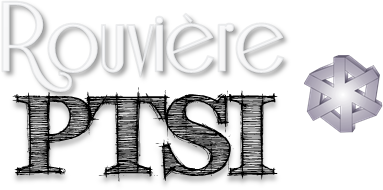
\includegraphics[width=2cm]{png/logo_ptsi.png}%
\end{minipage}
}

\fancyhead[C]{\rule{12cm}{.5pt}}

\fancyhead[R]{%
\begin{minipage}[c]{3cm}
\begin{flushright}
\footnotesize{\textit{\textsf{Sciences Industrielles\\ pour l'Ingénieur}}}%
\end{flushright}
\end{minipage}
}

\renewcommand{\footrulewidth}{0.2pt}

\fancyfoot[C]{\footnotesize{\bfseries \thepage}}
\fancyfoot[L]{\footnotesize{2012 -- 2013} \\ X. \textsc{Pessoles}}
\ifthenelse{\boolean{prof}}{%
\fancyfoot[R]{\footnotesize{Cours -- CI 2 : Cinématique -- P}}
}{%
\fancyfoot[R]{\footnotesize{Cours -- CI 2 : Cinématique}}
}

%\begin{center}
%\textit{Centre d'intérêt}
%\end{center}

\begin{center}
 \huge\textsc{CI 2 -- Cinématique : Modélisation, prévision et vérification du comportement cinématiques des systèmes}
\end{center}

\begin{center}
 \LARGE\textsc{Chapitre 3 -- Cinématique du point dans un mécanisme en mouvement} 
\end{center}

\vspace{.5cm}

\begin{center}
\begin{tabular}{ccccc}
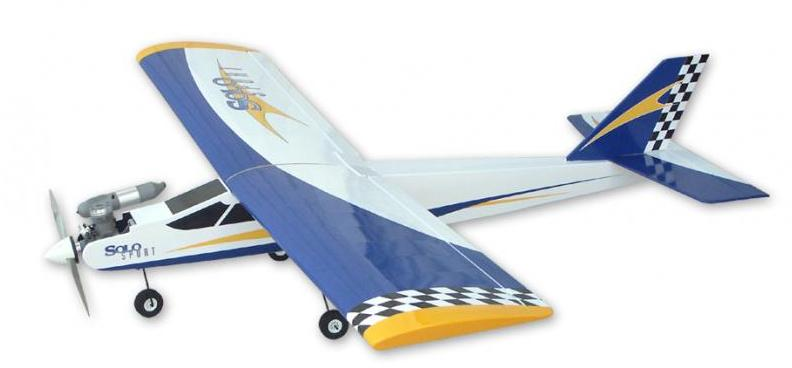
\includegraphics[height=2.5cm]{png/avion} &&
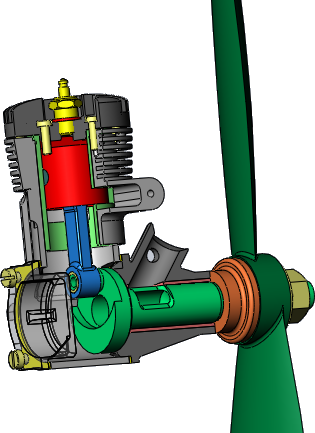
\includegraphics[height=3.5cm]{png/moteur_3d} && 
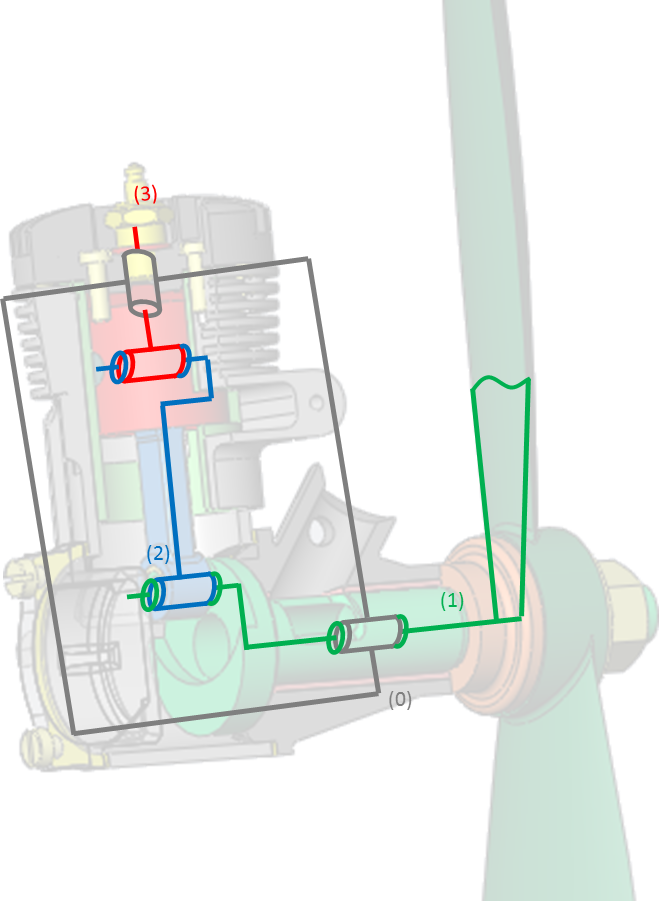
\includegraphics[height=3.5cm]{png/moteur_3d_sch}\\
\textit{Trainer Solo Sport \cite{cite1}} &&
\textit{Modèle CAO d'un} &&
\textit{Modélisation par}\\
 &&
\textit{moteur de modélisme \cite{cite2}} &&
\textit{schéma cinématique}\\
\end{tabular}
\end{center}

\vspace{.2cm}
L'étude des vitesses et des accélérations des points d'un solide est utile pour plusieurs raisons. En phase d'avant projet, par exemple, lors de la phase de conception d'un système mécanique de transmission ou de conversion de mouvement, il est indispensable de connaître la vitesse des solides afin de satisfaire à un cahier des charges.

En phase de dimensionnement des produits, certains composants peuvent être dimensionnés en fonction de la vitesse de fonctionnement du système. Dans d'autres cas, la cinématique est un préalable aux études de dynamique. 

\begin{prob}
\textsc{Problématique :}
\begin{itemize}
\item Comment déterminer le mouvement d'un solide dans un mécanisme complexe?
\end{itemize}
\end{prob}

\begin{savoir}
\textsc{Savoirs :}
\begin{itemize}
\item Connaître les propriétés du champ décrit par le vecteur vitesse
\item Déterminer le torseur traduisant le déplacement entre deux solides pour les liaisons connues
\end{itemize}
\end{savoir}

\setlength{\parskip}{0ex plus 0.2ex minus 0ex}
 \renewcommand{\contentsname}{}
 \renewcommand{\baselinestretch}{1}

% \vspace{1cm}
\textit{Ce document est en évolution permanente. Merci de signaler toutes
erreurs ou coquilles.}

\tableofcontents

 \renewcommand{\baselinestretch}{1.2}
\setlength{\parskip}{2ex plus 0.5ex minus 0.2ex}







\section{Champ décrit par le vecteur vitesse}
Dans le cadre de la conception des pièces constituants un mécanisme, il est nécessaire de connaître la vitesse en certains points qui constituent la pièce en plus des centres des liaisons. 
Cherchons donc la relation existant entre les vitesses de deux points appartenant à un solide en mouvement.


\begin{minipage}[c]{.65\linewidth}
Soit un solide $S_1$ en mouvement par rapport à un solide $S_0$. Soient $A$ et $B$ deux points appartenant à $S_1$. 

Calculons la dérivée du vecteur $\vect{AB}$ :
$$
\left[ \dfrac{d\vect{AB}}{dt}\right]_{\mathcal{R}_0} = 
\underbrace{\left[ \dfrac{d\vect{AB}}{dt}\right]_{\mathcal{R}_1}}_{\vect{0}} + \vect{\Omega(S_1/S_0)}\wedge \vect{AB}
=\vect{\Omega(S_1/S_0)}\wedge \vect{AB}
$$

Le point $O_1$ est un point fixe du mécanisme : en effet, $\vect{V(O_1\in S_1/S_0)}=\vect{0}$.

On a donc :
$$
\left[ \dfrac{d\vect{AB}}{dt}\right]_{\mathcal{R}_0} = 
\left[ \dfrac{d\vect{AO_1}}{dt}\right]_{\mathcal{R}_0} 
+\left[ \dfrac{d\vect{O_1B}}{dt}\right]_{\mathcal{R}_0}
=-\vect{V(A\in S_1/S_0)}+\vect{V(B\in S_1/S_0)}
$$
\end{minipage} \hfill
\begin{minipage}[c]{.3\linewidth}
\begin{center}
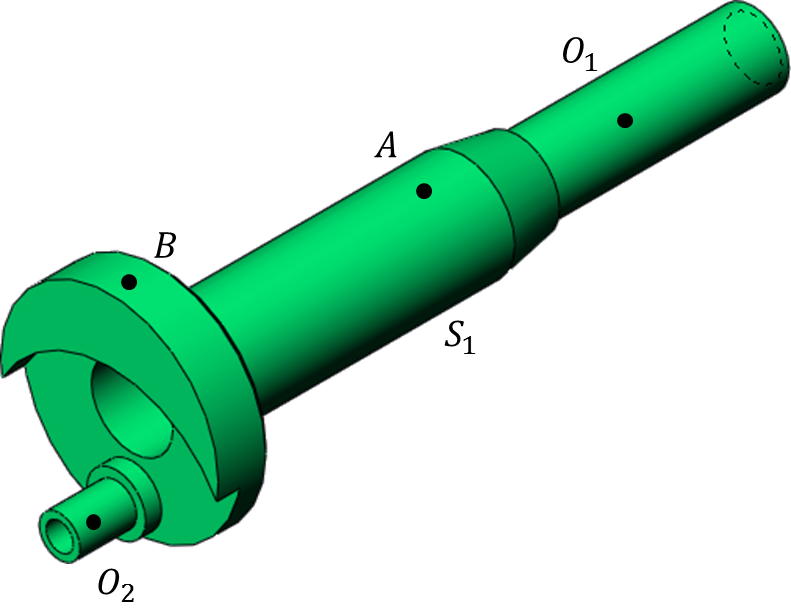
\includegraphics[width=.9\textwidth]{png/vilebrequin}
\end{center}
\end{minipage}

\vspace{.5cm}

En combinant les deux équations précédentes on obtient : 
$$
\vect{\Omega(S_1/S_0)}\wedge \vect{AB}=-\vect{V(A\in S_1/S_0)}+\vect{V(B\in S_1/S_0)}
$$
$$\Longleftrightarrow
\vect{V(B\in S_1/S_0)} = \vect{V(A\in S_1/S_0)} + \vect{\Omega(S_1/S_0)}\wedge \vect{AB}
$$
$$\Longleftrightarrow
\vect{V(B\in S_1/S_0)} = \vect{V(A\in S_1/S_0)} + \vect{BA}\wedge \vect{\Omega(S_1/S_0)}
$$

\subsection{Définition}
\begin{resultat}
\textbf{Champ du vecteur vitesse dans un solide}

Soient $A$ et $B$ deux points appartenant à un solide $S_1$ en mouvement par rapport à $S_0$. Le champ des vecteurs vitesses est donc déterminé ainsi :
$$
\vect{V(B\in S_1/S_0)} = \vect{V(A\in S_1/S_0)} + \vect{BA}\wedge \vect{\Omega(S_1/S_0)}
$$
\end{resultat}

\begin{rem}

\textit{Moyen mnémotechnique}

\begin{minipage}[c]{.65\linewidth}
Comme la dérivée vectorielle, l'utilisation de cette formule est indispensable en mécanique en général et en cinématique en particulier.

On verra par la suite que le vecteur $\vect{\Omega}$ est appelé \textbf{R}ésultante du torseur cinématique. 

En conséquence, en utilisant le moyen mnémotechnique on a :
$$
\vect{V(\mathbf{B}\in S_1/S_0)} = \vect{V(\mathbf{A}\in S_1/S_0)} + \vect{\mathbf{BA}}\wedge \underbrace{\vect{\Omega(S_1/S_0)}}_{\mathbf{R}}
$$
\end{minipage}
\begin{minipage}[c]{.3\linewidth}
\begin{center}

\includegraphics[width=.6\textwidth]{png/babar}
\end{center}
\end{minipage}
\end{rem}

\begin{rem}
\textit{Utilisation du champ de vecteur}

La formule du champ de vecteur est utilisée à chaque fois que la vitesse est connue en un point d'un solide et qu'on veut la calculer en un point appartenant à un autre point d'un même solide. 
\end{rem}

\begin{exemple}
\begin{center}
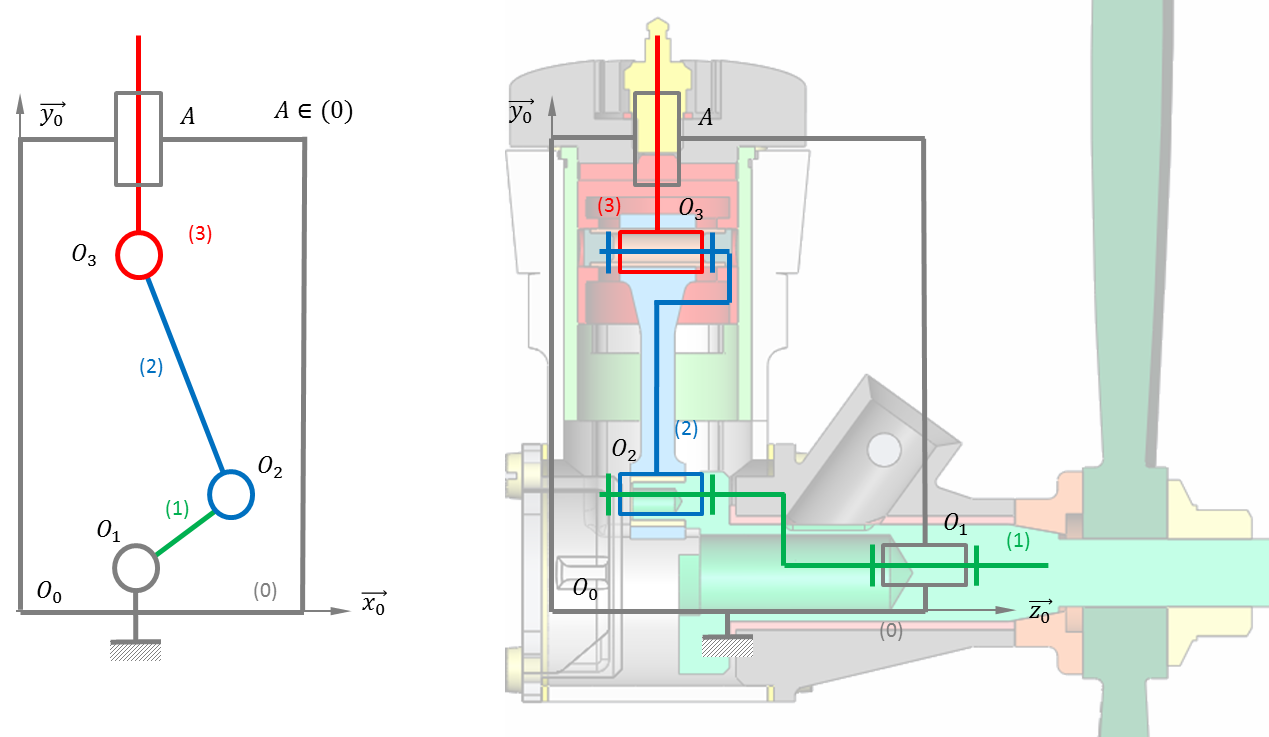
\includegraphics[width=.8\textwidth]{png/moteur_2d_sch}

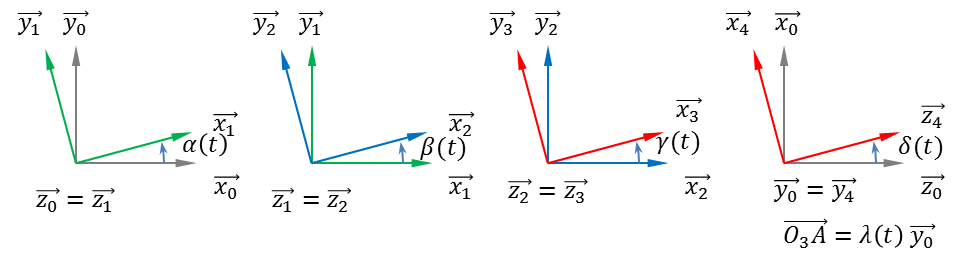
\includegraphics[width=\textwidth]{png/param}
\end{center}
\textit{Calculer $\vectv{O_2}{S_2}{S_0}$}

\vspace{5cm}

\end{exemple}
\subsection{Equiprojectivité du champ des vecteurs vitesses}
\begin{resultat}
\textbf{Equiprojectivité}

Soit un solide $S_1$ en mouvement par rapport à un repère fixe $\mathcal{R}_0$. Soient deux points $A$ et $B$ appartenant au solide $S_1$. On démontre qu'à chaque instant $t$ :
$$
\vectv{A}{S_1}{\mathcal{R}_0}\cdot \vect{AB} = 
\vectv{B}{S_1}{\mathcal{R}_0}\cdot \vect{AB}
$$
\end{resultat}

\begin{rem}
Cette propriété sera très utilisée en cinématique graphique lors de l'étude des mouvements plans.
\end{rem}

\subsection{Cas particuliers de mouvements élémentaires}
\subsubsection{Solide en rotation autour d'un axe fixe}

Soit $S$ un solide en rotation autour d'un axe fixe ($\Delta$) par rapport à $\mathcal{R}$. $\Delta$ est appelé axe instantané de rotations. Pour tout point $P$ appartenant à $\Delta$, on a : 
$$\vectv{P}{S}{\mathcal{R}}=\vect{0}$$

%\begin{exemple}
%\end{exemple}


\subsubsection{Solide en translation -- Liaison glissière}

Soit $S$ un solide en translation suivant un axe fixe (axe dirigé par $\vect{u}$) par rapport à $\mathcal{R}$. Pour tout point $P_1$ et $P_2$ appartenant à $S$, on a : 
$$
\vectv{P_1}{S}{\mathcal{R}_0}=\vectv{P_2}{S}{\mathcal{R}_0}
$$


%\begin{exemple}
%\end{exemple}
%\subsubsection{Solide en translation hélicoïdale}


\section{Torseur cinématique entre deux solides}
\subsection{Définition}
La vitesse d'un solide par rapport à un autre solide peut être exprimée par 
\begin{itemize}
\item le vecteur vitesse en un point qui traduit la vitesse de translation du solide;
\item le vecteur instantané de rotation qui traduit la vitesse de rotation du solide.
\end{itemize}

\begin{defi}
\textbf{Torseur cinématique}

Le torseur permet d'écrire sous forme réduite les vecteurs vitesses d'un solide. Ainsi le torseur cinématique entre les solides $S_1$ et $S_0$ s'exprime ainsi :
$$
\torseurcin{V}{S_1}{S_0} = \torseurl{\vecto{S_1}{S_0}}{\vectv{A}{S_1}{S_0}}{A}
$$
\end{defi}

\begin{rem}
\begin{itemize}
\item Lors de l'écriture en ligne d'un torseur, il est obligatoire de préciser le point d'application.
\item $\vecto{S_1}{S_0}$ est appelé résultante du torseur cinématique. La résultante est indépendante du point d'application. 
\item $\vectv{A}{S_1}{S_0}$ est appelé le moment du torseur cinématique. Il dépend du point d'application.
\item Un torseur est un objet mathématique que l'on peut noter :
$$
\torseur{\mathcal{T}} = \torseurl{\vect{R}}{\vect{\mathcal{M}(A)}}{A}
$$
\end{itemize}
\end{rem}
\subsection{Propriétés}
\begin{prop}
\textbf{Égalité entre torseurs}

Deux torseurs $\torseur{\mathcal{T}_1}$ et $\torseur{\mathcal{T}_2}$ sont égaux si et seulement si:
\begin{itemize}
\item $\vect{R_1} = \vect{R_2}$
\item il existe un point $A$ tel que 
$\vect{\mathcal{M}_{1}(A)} = \vect{\mathcal{M}_{2}(A)}$
\end{itemize}
\end{prop}

\begin{prop}
\textbf{Égalité entre torseurs}

Deux torseurs $\torseur{\mathcal{T}_1}$ et $\torseur{\mathcal{T}_2}$ sont égaux si et seulement si:
\begin{itemize}
\item $\vect{R_1} = \vect{R_2}$
\item il existe un point $A$ tel que 
$\vect{\mathcal{M}_{1}(A)} = \vect{\mathcal{M}_{2}(A)}$
\end{itemize}
\end{prop}

\begin{defi}
\textbf{Co moment de torseurs}

Le co moment de deux torseurs $\torseur{\mathcal{T}_1}$ et $\torseur{\mathcal{T}_2}$ est défini par : 
$$
\torseur{\mathcal{T}_1} \otimes \torseur{\mathcal{T}_2} = 
\vect{R_1} \cdot \vect{\mathcal{M}_{2}(A)} + 
\vect{R_2} \cdot \vect{\mathcal{M}_{1}(A)}
$$
\begin{itemize}
\item Le résultat de cette opération est un nombre réel.
\item L'opération doit être réalisée lorsque les deux torseurs sont au même point. 
\item Le résultat de l'opération est indépendant du point d'application.
\item Le co moment du torseur cinématique et du torseur statique exprime la puissance.
\end{itemize}
\end{defi}

\begin{defi}
\textbf{Point central}

Le point central d'un torseur est un point pour lequel la résultante et le moment sont colinéaires.
\end{defi}


\begin{resultat}
\textbf{Axe central}

L'axe central $\Delta$ d'un torseur est la droite sur laquelle sont situés tous les points centraux. 

On montre que :
\begin{itemize}
\item la direction de l'axe central a la même direction que la résultante du torseur;
\item si on note $H$ le projeté orthogonal de $A$ sur $\Delta$, alors $\vect{AH}=\dfrac{\vect{R}\wedge \vect{\mathcal{M}(A)}}{\vect{R}^2}$;
\item le moment en tout point de l'axe central est minimal et vaut : 
$\vect{\mathcal{M}(H)}=\dfrac{\vect{R}\cdot \vect{\mathcal{M}(A)}}{\vect{R}^2}\cdot\vect{R}
$.
\end{itemize}
\end{resultat}

\subsection{Torseur remarquables}
\begin{defi}
\textbf{Torseur couple}

Un torseur est dit "torseur couple" lorsque la résultante du torseur est nulle et lorsque le moment est non nul :
$$
\torseur{\mathcal{T}} = \torseurl{\vect{0}}{\vect{\mathcal{M}(A)}}{A}
$$

L'axe central d'un torseur couple n'existe pas.
\end{defi}


\begin{defi}
\textbf{Torseur glisseur}

Un torseur est dit "glisseur" lorsque la résultante du torseur est non nulle et lorsque l'automoment est nul :
$$
\torseur{\mathcal{T}} = \torseurl{\vect{R}}{\vect{\mathcal{M}(A)}}{A} \text{ avec } \forall A, 
\vect{R} \cdot \vect{\mathcal{M}(A)} = 0
$$ 

On montre alors que sur tout point $K$ de l'axe central, 
$$
\torseur{\mathcal{T}} = \torseurl{\vect{R}}{\vect{0}}{K}
$$

\end{defi}
\subsection{Torseur cinématique des liaisons usuelles}

\begin{center}
\begin{tabular}{|p{.15\textwidth}|p{.1\textwidth}|p{.1\textwidth}|p{.1\textwidth}|p{.22\textwidth}|}
\hline
 & 
\begin{center}
Schémas plans
\end{center} & 
\begin{center}
Schéma spatial
\end{center} & 
\begin{center}
DDL 
\end{center}& 
\begin{center}
Torseur cinématique 
\end{center} \\
\hline
\hline
\begin{center}
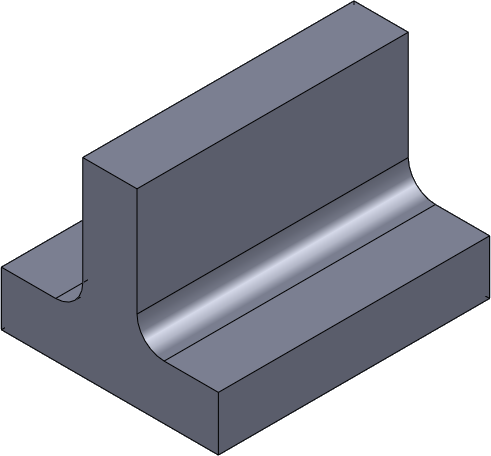
\includegraphics[height=1.5cm]{png/encastrement}
\end{center}
& & &  
&$$\torseurc{\mathcal{V}\left(S_2/S_1\right)}{\quad}{}{}{}{}{}{\_}$$\\
\hline
\begin{center}
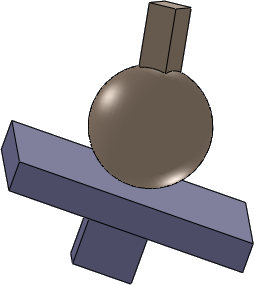
\includegraphics[height=1.5cm]{png/ponctuelle}
\end{center}
& & & 
&$$\torseurc{\mathcal{V}\left(S_2/S_1\right)}{\quad}{}{}{}{}{}{\_}$$\\
\hline
\begin{center}
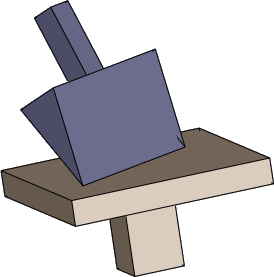
\includegraphics[height=1.5cm]{png/rectiligne}
\end{center}
& & & 
&$$\torseurc{\mathcal{V}\left(S_2/S_1\right)}{\quad}{}{}{}{}{}{\_}$$\\
\hline
\begin{center}
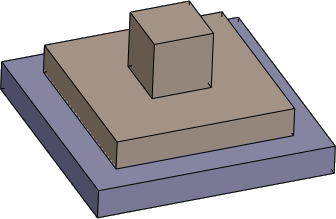
\includegraphics[height=1.5cm]{png/plan}
\end{center}
& & & 
&$$\torseurc{\mathcal{V}\left(S_2/S_1\right)}{\quad}{}{}{}{}{}{\_}$$\\
\hline
\begin{center}
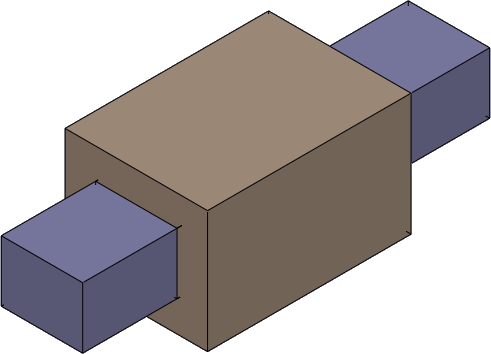
\includegraphics[height=1.5cm]{png/glissiere}
\end{center}
& & & 
&$$\torseurc{\mathcal{V}\left(S_2/S_1\right)}{\quad}{}{}{}{}{}{\_}$$\\
\hline
\end{tabular}
\end{center}



\begin{center}
\begin{tabular}{|p{.15\textwidth}|p{.1\textwidth}|p{.1\textwidth}|p{.1\textwidth}|p{.22\textwidth}|}
\hline
 & 
\begin{center}
Schémas plans
\end{center} & 
\begin{center}
Schéma spatial
\end{center} & 
\begin{center}
DDL 
\end{center}& 
\begin{center}
Torseur cinématique 
\end{center} \\
\hline
\hline
\begin{center}
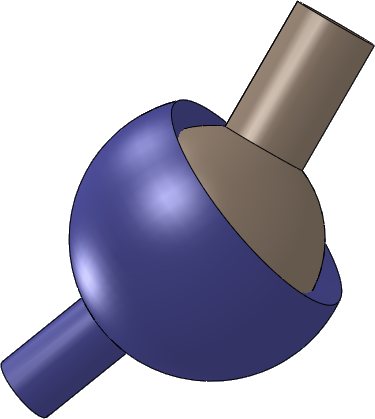
\includegraphics[height=1.5cm]{png/rotule}
\end{center}
& & &  
&$$\torseurc{\mathcal{V}\left(S_2/S_1\right)}{\quad}{}{}{}{}{}{\_}$$\\
\hline
\begin{center}
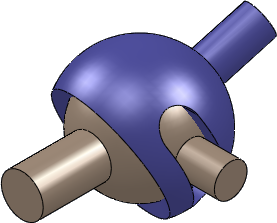
\includegraphics[height=1.5cm]{png/rotuled}
\end{center}
& & & 
&$$\torseurc{\mathcal{V}\left(S_2/S_1\right)}{\quad}{}{}{}{}{}{\_}$$\\
\hline
\begin{center}
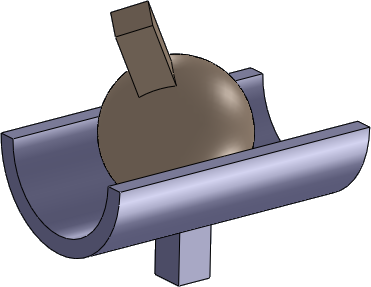
\includegraphics[height=1.5cm]{png/lineaire}
\end{center}
& & & 
&$$\torseurc{\mathcal{V}\left(S_2/S_1\right)}{\quad}{}{}{}{}{}{\_}$$\\
\hline
\begin{center}
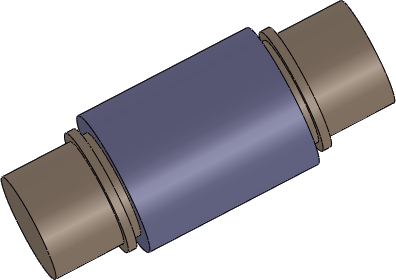
\includegraphics[height=1.5cm]{png/pivot}
\end{center}
& & & 
&$$\torseurc{\mathcal{V}\left(S_2/S_1\right)}{\quad}{}{}{}{}{}{\_}$$\\
\hline
\begin{center}
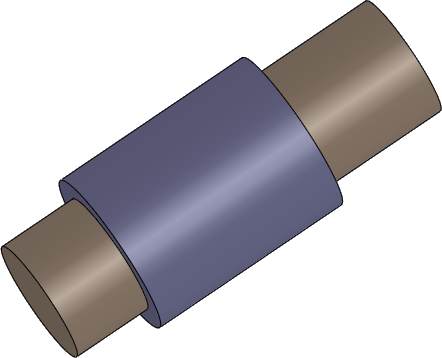
\includegraphics[height=1.5cm]{png/pivotg}
\end{center}
& & & 
&$$\torseurc{\mathcal{V}\left(S_2/S_1\right)}{\quad}{}{}{}{}{}{\_}$$\\
\hline
\begin{center}
Liaison glissière hélicoïdale
%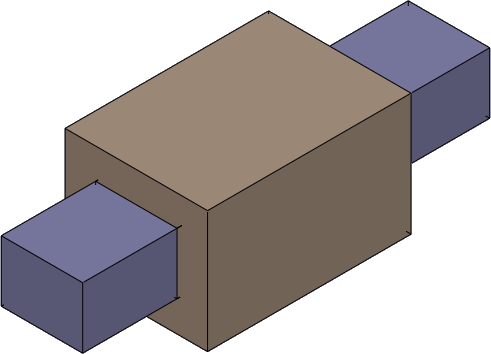
\includegraphics[height=1.5cm]{png/glissiere}
\end{center}
& & & 
&$$\torseurc{\mathcal{V}\left(S_2/S_1\right)}{\quad}{}{}{}{}{}{\_}$$\\
\hline
\end{tabular}
\end{center}

\subsection{Exemple}
\begin{exemple}
Donner le torseur associé à chacune des liaisons :

$$ \torseur{\mathcal{V}(S_1/S_0)} =\torseurl{\vecto{S_1}{S_0}=}{\vectv{O_1}{S_1}{S_0}=\quad \quad \quad \quad \quad \quad \quad \quad \quad \quad \quad}{O_1}
$$

$$ \torseur{\mathcal{V}(S_1/S_0)} =\torseurl{\vecto{S_1}{S_0}=}{\vectv{O_2}{S_1}{S_0}=\quad \quad \quad \quad \quad \quad \quad \quad \quad \quad \quad}{O_2}
$$

$$ \torseur{\mathcal{V}(S_2/S_1)} =\torseurl{\vecto{S_2}{S_1}=}{\vectv{O_2}{S_2}{S_1}=\quad \quad \quad \quad \quad \quad \quad \quad \quad \quad \quad}{O_2}
$$

$$ \torseur{\mathcal{V}(S_3/S_2)} =\torseurl{\vecto{S_3}{S_2}=}{\vectv{O_3}{S_3}{S_2}=\quad \quad \quad \quad \quad \quad \quad \quad \quad \quad \quad}{O_3}
$$

$$ \torseur{\mathcal{V}(S_3/S_0)} =\torseurl{\vecto{S_3}{S_0}=}{\vectv{A}{S_3}{S_0}=\quad \quad \quad \quad \quad \quad \quad \quad \quad \quad \quad}{A}
$$

\end{exemple}

\section{Composition des mouvements}
\subsection{Composition du vecteur vitesse}
\begin{resultat}
\textbf{Composition du vecteur vitesse}
\label{ref_va}
Soit un solide $S_1$ en mouvement par rapport à un repère $\mathcal{R}_0$ et un solide $S_2$ par rapport au solide $S_1$. Pour chacun des points $A$ appartenant au solide $S_2$, on a :
$$
\vectv{A}{S_2}{\mathcal{R}_0}=
\vectv{A}{S_2}{S_1}+\vectv{A}{S_1}{\mathcal{R}_0}
$$
\end{resultat}

Démontrons ce résultat. $O_1$ est le centre de la liaison entre $\mathcal{R}_0$ et $S_1$. $O_1$ est donc fixe dans le repère $\mathcal{R}_0$. $O_2$ est le centre de la liaison entre $S_1$ et $S_2$. $A$ appartient à $S_2$. 
$$
\vectv{A}{S_2}{\mathcal{R}_0}
= \left[\dfrac{\vect{dO_1 A}}{dt}
\right]_{\mathcal{R}_0}
= \left[\dfrac{\vect{dO_1 O_2}}{dt}
\right]_{\mathcal{R}_0}
+
\left[\dfrac{\vect{dO_2 A}}{dt}
\right]_{\mathcal{R}_0}
=
\vectv{O_2}{S_1}{\mathcal{R}_0}
+
\left[\dfrac{\vect{dO_2 A}}{dt}\right]_{S_1}
+\vecto{S_1}{\mathcal{R}_0}\wedge \vect{O_2 A}
$$

$$
\vectv{A}{S_2}{\mathcal{R}_0}
=
\underbrace{\left[\dfrac{\vect{dO_2 A}}{dt}\right]_{S_1}}_{\vectv{A}{S_2}{S_1}}
+
\underbrace{\vectv{O_2}{S_1}{\mathcal{R}_0}
+
\vect{AO_2}
\wedge 
\vecto{S_1}{\mathcal{R}_0}}_{\vectv{A}{S_1}{\mathcal{R}_0}}
$$


On a donc bien : 
$$
\vectv{A}{S_2}{\mathcal{R}_0}
=
\vectv{A}{S_2}{S_1}
+
\vectv{A}{S_1}{\mathcal{R}_0}
$$

\begin{rem}
\begin{itemize}
\item $\vectv{A}{S_2}{\mathcal{R}_0}$ est appelé vecteur vitesse absolu;
\item $\vectv{A}{S_2}{S_1}$ est appelé vecteur vitesse relatif; 
\item $\vectv{A}{S_1}{\mathcal{R}_0}$ est appelé vecteur vitesse d'entraînement.
\end{itemize}
\end{rem}

\begin{resultat}
\textbf{Généralisation}

La décomposition du vecteur vitesse peut se généraliser avec $n$ solides : 
$$
\vectv{A}{S_n}{S_0}
=
\vectv{A}{S_n}{S_{n-1}}
+...+
\vectv{A}{S_1}{S_0}
$$

\end{resultat}

\subsection{Composition du vecteur instantané de rotation}
\begin{resultat}
\textbf{Composition du vecteur vitesse}

Soit un solide $S_1$ en mouvement par rapport à un repère $\mathcal{R}_0$ et un solide $S_2$ par rapport au solide $S_1$. On a : 
$$
\vecto{S_2}{\mathcal{R}_0}=
\vecto{S_2}{S_1}+\vecto{S_1}{\mathcal{R}_0}
$$
\end{resultat}

Pour démontrer ce résultat, prenons un vecteur $\vect{v}$ :
$$
\left[\dfrac{d\vect{v}}{dt}\right]_{S_1} = 
\left[\dfrac{d\vect{v}}{dt}\right]_{S_2} 
+ \vecto{S_2}{S_1} \wedge \vect{v}
$$

$$
\left[\dfrac{d\vect{v}}{dt}\right]_{S_1} = 
\left[\dfrac{d\vect{v}}{dt}\right]_{\mathcal{R}_0} 
+ \vecto{\mathcal{R}_0}{S_1} \wedge \vect{v}
$$

$$
\left[\dfrac{d\vect{v}}{dt}\right]_{\mathcal{R}_0} = 
\left[\dfrac{d\vect{v}}{dt}\right]_{S_2} 
+ \vecto{S_2}{\mathcal{R}_0} \wedge \vect{v} \Longleftrightarrow 
\left[\dfrac{d\vect{v}}{dt}\right]_{\mathcal{R}_0} 
-\left[\dfrac{d\vect{v}}{dt}\right]_{S_2} 
= \vecto{S_2}{\mathcal{R}_0} \wedge \vect{v}
$$

En faisant la soustraction des deux premières expressions on obtient : 
$$
\vect{0} = 
\left[\dfrac{d\vect{v}}{dt}\right]_{S_2} 
-\left[\dfrac{d\vect{v}}{dt}\right]_{\mathcal{R}_0} 
+ \vecto{S_2}{S_1} \wedge \vect{v}
- \vecto{\mathcal{R}_0}{S_1} \wedge \vect{v}
=\left[\dfrac{d\vect{v}}{dt}\right]_{S_2} 
-\left[\dfrac{d\vect{v}}{dt}\right]_{\mathcal{R}_0} 
+ \left(\vecto{S_2}{S_1} - \vecto{\mathcal{R}_0}{S_1}  \right)\wedge \vect{v}
$$

$$
\Longleftrightarrow
\left[\dfrac{d\vect{v}}{dt}\right]_{\mathcal{R}_0} 
-\left[\dfrac{d\vect{v}}{dt}\right]_{S_2} 
=
 \left(\vecto{S_2}{S_1} + \vecto{S_1}{\mathcal{R}_0}  \right)\wedge \vect{v}
$$
En utilisant la dernière relation on a donc : 
$$
\vecto{S_2}{\mathcal{R}_0} \wedge \vect{v}
=
 \left(\vecto{S_2}{S_1} + \vecto{S_1}{\mathcal{R}_0}  \right)\wedge \vect{v}
\Longleftrightarrow
\vecto{S_2}{\mathcal{R}_0} = \vecto{S_2}{S_1} + \vecto{S_1}{\mathcal{R}_0}
$$
\begin{resultat}
\textbf{Généralisation}

La décomposition du vecteur instantané de rotation peut se généraliser avec $n$ solides : 
$$
\vecto{S_n}{S_0}
=
\vecto{S_n}{S_{n-1}}
+...+
\vecto{S_1}{S_0}
$$
\end{resultat}

\subsection{Composition du torseur cinématique}
\begin{resultat}
\textbf{Décomposition du torseur cinématique}

Des parties précédentes, on peut conclure qu'on peut décomposer le torseur cinématique : 

$$
\torseurcin{V}{S_n}{S_0} = 
\torseurcin{V}{S_n}{S_{n-1}} +... +\torseurcin{V}{S_1}{S_0}
$$

Ou encore : 

$$
\torseurl{\vecto{S_n}{S_0}}{\vectv{A}{S_n}{S_0}}{A}=
\torseurl{\vecto{S_n}{S_{n-1}}}{\vectv{A}{S_n}{S_{n-1}}}{A}
+...+
\torseurl{\vecto{S_1}{S_0}}{\vectv{A}{S_1}{S_0}}{A}
$$

\end{resultat}

\begin{exemple}
\textit{Donner le torseur $\torseur{\mathcal{V}(S_2/S_0)}$.}
\end{exemple}

\section{Accélération d'un solide}
\subsection{Champ d'accélération d'un solide en mouvement}
On a vu que 
$\vectv{B}{S_1}{S_0} = \vectv{A}{S_1}{S_0} + \vect{BA} \wedge \vecto{S_1}{S_0}$. En dérivant cette expression on a donc : 
$$
\vectg{B}{S_1}{S_0} 
= \vectg{A}{S_1}{S_0} 
+\left[\dfrac{d\vect{BA}}{dt}\right]_{S_0} \wedge \vecto{S_1}{S_0}
+\vect{BA} \wedge \left[\dfrac{d\vecto{S_1}{S_0}}{dt}\right]_{S_0}
$$

$B$ et $A$ sont des points du solide $S_1$. On a donc : 
 $$
\left[\dfrac{d\vect{BA}}{dt}\right]_{S_0} =
\underbrace{\left[\dfrac{d\vect{BA}}{dt}\right]_{S_1}}_{\vect{0}} 
+ \vecto{S_1}{S_0} \wedge \vect{BA}
$$

$$
\vectg{B}{S_1}{S_0} 
= \vectg{A}{S_1}{S_0} 
+\vecto{S_1}{S_0} \wedge \vect{BA}
\wedge \vecto{S_1}{S_0}
+\vect{BA} \wedge \left[\dfrac{d\vecto{S_1}{S_0}}{dt}\right]_{S_0}
$$

$$
\vectg{B}{S_1}{S_0} 
= \vectg{A}{S_1}{S_0} 
+\vecto{S_1}{S_0} \wedge \vecto{S_1}{S_0}
\wedge \vect{AB}
+\left[\dfrac{d\vecto{S_1}{S_0}}{dt}\right]_{S_0} \wedge \vect{AB} 
$$

\begin{resultat}
Le champ des accélérations n'est donc pas un champ de moment.
\end{resultat}

\subsection{Composition des accélérations}
On a vu que la vitesse d'un solide $S_2$ par rapport à $\mathcal{R}_0$ au point $A$ pouvait s'exprimer ainsi (paragraphe \ref{ref_va}, page \pageref{ref_va}):

$$
\vectv{A}{S_2}{\mathcal{R}_0}
=
\underbrace{\left[\dfrac{\vect{dO_2 A}}{dt}\right]_{S_1}}_{\vectv{A}{S_2}{S_1}}
+
\underbrace{\vectv{O_2}{S_1}{\mathcal{R}_0}
+
\vect{AO_2}
\wedge 
\vecto{S_1}{\mathcal{R}_0}}_{\vectv{A}{S_1}{\mathcal{R}_0}}
$$
$$
\Longleftrightarrow
\vectv{A}{S_2}{\mathcal{R}_0}
=
\vectv{A}{S_2}{S_1} + \vectv{O_2}{S_1}{\mathcal{R}_0}
+
\vect{AO_2}
\wedge 
\vecto{S_1}{\mathcal{R}_0}
$$

Calculons l'accélération du point : 
$$
\vectg{A}{S_2}{\mathcal{R}_0}=
\left[
\dfrac{d\vectv{A}{S_2}{\mathcal{R}_0}}{dt}
\right]_{\mathcal{R}_0}
$$

$$
\vectg{A}{S_2}{\mathcal{R}_0}
=
\left[
\dfrac{d
\vectv{A}{S_2}{S_1} }{dt}
\right]_{\mathcal{R}_0}
+ 
\left[
\dfrac{d\vectv{O_2}{S_1}{\mathcal{R}_0}}{dt}
\right]_{\mathcal{R}_0}
+
\left[
\dfrac{d\vect{AO_2}}{dt}
\right]_{\mathcal{R}_0}
\wedge 
\vecto{S_1}{\mathcal{R}_0}
+
\vect{AO_2}
\wedge 
\left[
\dfrac{d\vecto{S_1}{\mathcal{R}_0}}{dt}
\right]_{\mathcal{R}_0}
$$


$$
\left[
\dfrac{d
\vectv{A}{S_2}{S_1} }{dt}
\right]_{\mathcal{R}_0}
=
\left[
\dfrac{d
\vectv{A}{S_2}{S_1} }{dt}
\right]_{S_1}
+
\vecto{S_2}{\mathcal{R}_0}\wedge\vectv{A}{S_2}{S_1}
$$

$$
\Longleftrightarrow
\left[
\dfrac{d
\vectv{A}{S_2}{S_1} }{dt}
\right]_{\mathcal{R}_0}
=
\vectg{A}{S_2}{S_1} 
+
\vecto{S_2}{\mathcal{R}_0}\wedge\vectv{A}{S_2}{S_1}
$$


$$
\left[
\dfrac{d\vectv{O_2}{S_1}{\mathcal{R}_0}}{dt}
\right]_{\mathcal{R}_0} 
= \vectg{O_2}{S_1}{\mathcal{R}_0}
$$

$$
\left[
\dfrac{d\vect{AO_2}}{dt}
\right]_{\mathcal{R}_0}
=
\left[
\dfrac{d\vect{AO_2}}{dt}
\right]_{S_1}
+
\vecto{S_1}{\mathcal{R}_0}
\wedge 
\vect{AO_2}
=
\vectv{A}{S_2}{S_1}+
\vecto{S_1}{\mathcal{R}_0}
\wedge 
\vect{AO_2}
$$


On a donc : 
\begin{eqnarray*}
\vectg{A}{S_2}{\mathcal{R}_0}
&=&
\vectg{A}{S_2}{S_1} + \vecto{S_2}{\mathcal{R}_0}\wedge\vectv{A}{S_2}{S_1}
+\vectg{O_2}{S_1}{\mathcal{R}_0}
+\vectv{A}{S_2}{S_1\wedge \vecto{S_1}{\mathcal{R}_0}}\\
&+&\vecto{S_1}{\mathcal{R}_0} \wedge \vecto{S_1}{\mathcal{R}_0} \wedge \vect{O_2A}
+
\left[
\dfrac{d\vecto{S_1}{\mathcal{R}_0}}{dt}
\right]_{\mathcal{R}_0}
\wedge 
\vect{O_2A}
\end{eqnarray*}

Par ailleurs d'après le paragraphe précédent, 
$$
\vectg{A}{S_1}{\mathcal{R}_0} 
= \vectg{O_2}{S_1}{\mathcal{R}_0} 
+\vecto{S_1}{\mathcal{R}_0} \wedge \vecto{S_1}{\mathcal{R}_0}
\wedge \vect{O_2A}
+\left[\dfrac{d\vecto{S_1}{\mathcal{R}_0}}{dt}\right]_{\mathcal{R}_0} \wedge \vect{O_2A} 
$$

Au final, 
$$
\vectg{A}{S_2}{\mathcal{R}_0}
=
\vectg{A}{S_2}{S_1} + \underbrace{2\vecto{S_2}{\mathcal{R}_0}}_{\vectg{A}{S_1}{\mathcal{R}_0}_{Cor}}\wedge\vectv{A}{S_2}{S_1}
+\vectg{A}{S_1}{\mathcal{R}_0} 
$$


\begin{resultat}
On ne peut donc pas composer les vitesses.
On appelle : 
\begin{itemize}
\item $\vectg{A}{S_2}{\mathcal{R}_0}$ : accélération absolue;
\item $\vectg{A}{S_2}{S_1}$ : accélération relative;
\item $\vectg{A}{S_1}{\mathcal{R}_0}$ : accélération absolue;
\item $\vectg{A}{S_1}{\mathcal{R}_0}_{Cor}$ : accélération de Coriolis.
\end{itemize}
\end{resultat}

\begin{thebibliography}{2}
  \bibitem[1]{cite1} Trainer Solo Sport, \textit{Avio et Tiger}, \url{http://www.net-loisirs.com/trainer-solo-sport-p1155.html}.

\bibitem[2]{cite2} Université Bretagne Sud, \textit{Moteur de modélisme} \url{http://foad.univ-ubs.fr/file.php/1355/TP_meca3d/Moteur_modelisme.zip}

\bibitem[3]{cite3} \url{http://www.aquadesign.be/actu/article-2535.php}
\end{thebibliography}
\end{document}
